\documentclass{beamer}

\usepackage{color}
\usepackage{graphicx}
\usepackage{geometry}
\usepackage{url}
\usepackage{pgfpages}
\usepackage{color}
\usepackage{ifthen}
\usetheme{Berlin}
\usecolortheme{ufrn}

\title[Turks in Germany]{Ausl{\"a}nder}
\date{\today}
\author{Brennan W. Fieck}
\institute{LAIS 418 - Narrating the Notion}

\setbeamertemplate{headline}
{%
	\begin{beamercolorbox}[colsep=1.5pt]{upper separation line head}
	\end{beamercolorbox}
	\begin{beamercolorbox}{section in head/foot}
		\vskip2pt\insertnavigation{paperwidth}\vskip2pt
	\end{beamercolorbox}%
	\begin{beamercolorbox}[colsep=1.5pt]{lower separation line head}
	\end{beamercolorbox}
}

\begin{document}
\frame{\titlepage}
\section{}
\begin{frame}{Summary}
	\tableofcontents
\end{frame}

\section{Early Incursions}
\begin{frame}{Early Incursions}
	\begin{columns}
		\column{0.6\textwidth}
			\begin{enumerate}
				\item Sieges of Vienna (1529, 1683)
				\item Great Turkish War (1683-1699)
				\item Prussian Soldiers (mid 1700's)
			\end{enumerate}
		\column{0.4\textwidth}
			\vcenter
			\begin{figure}[ht]
				\centering
				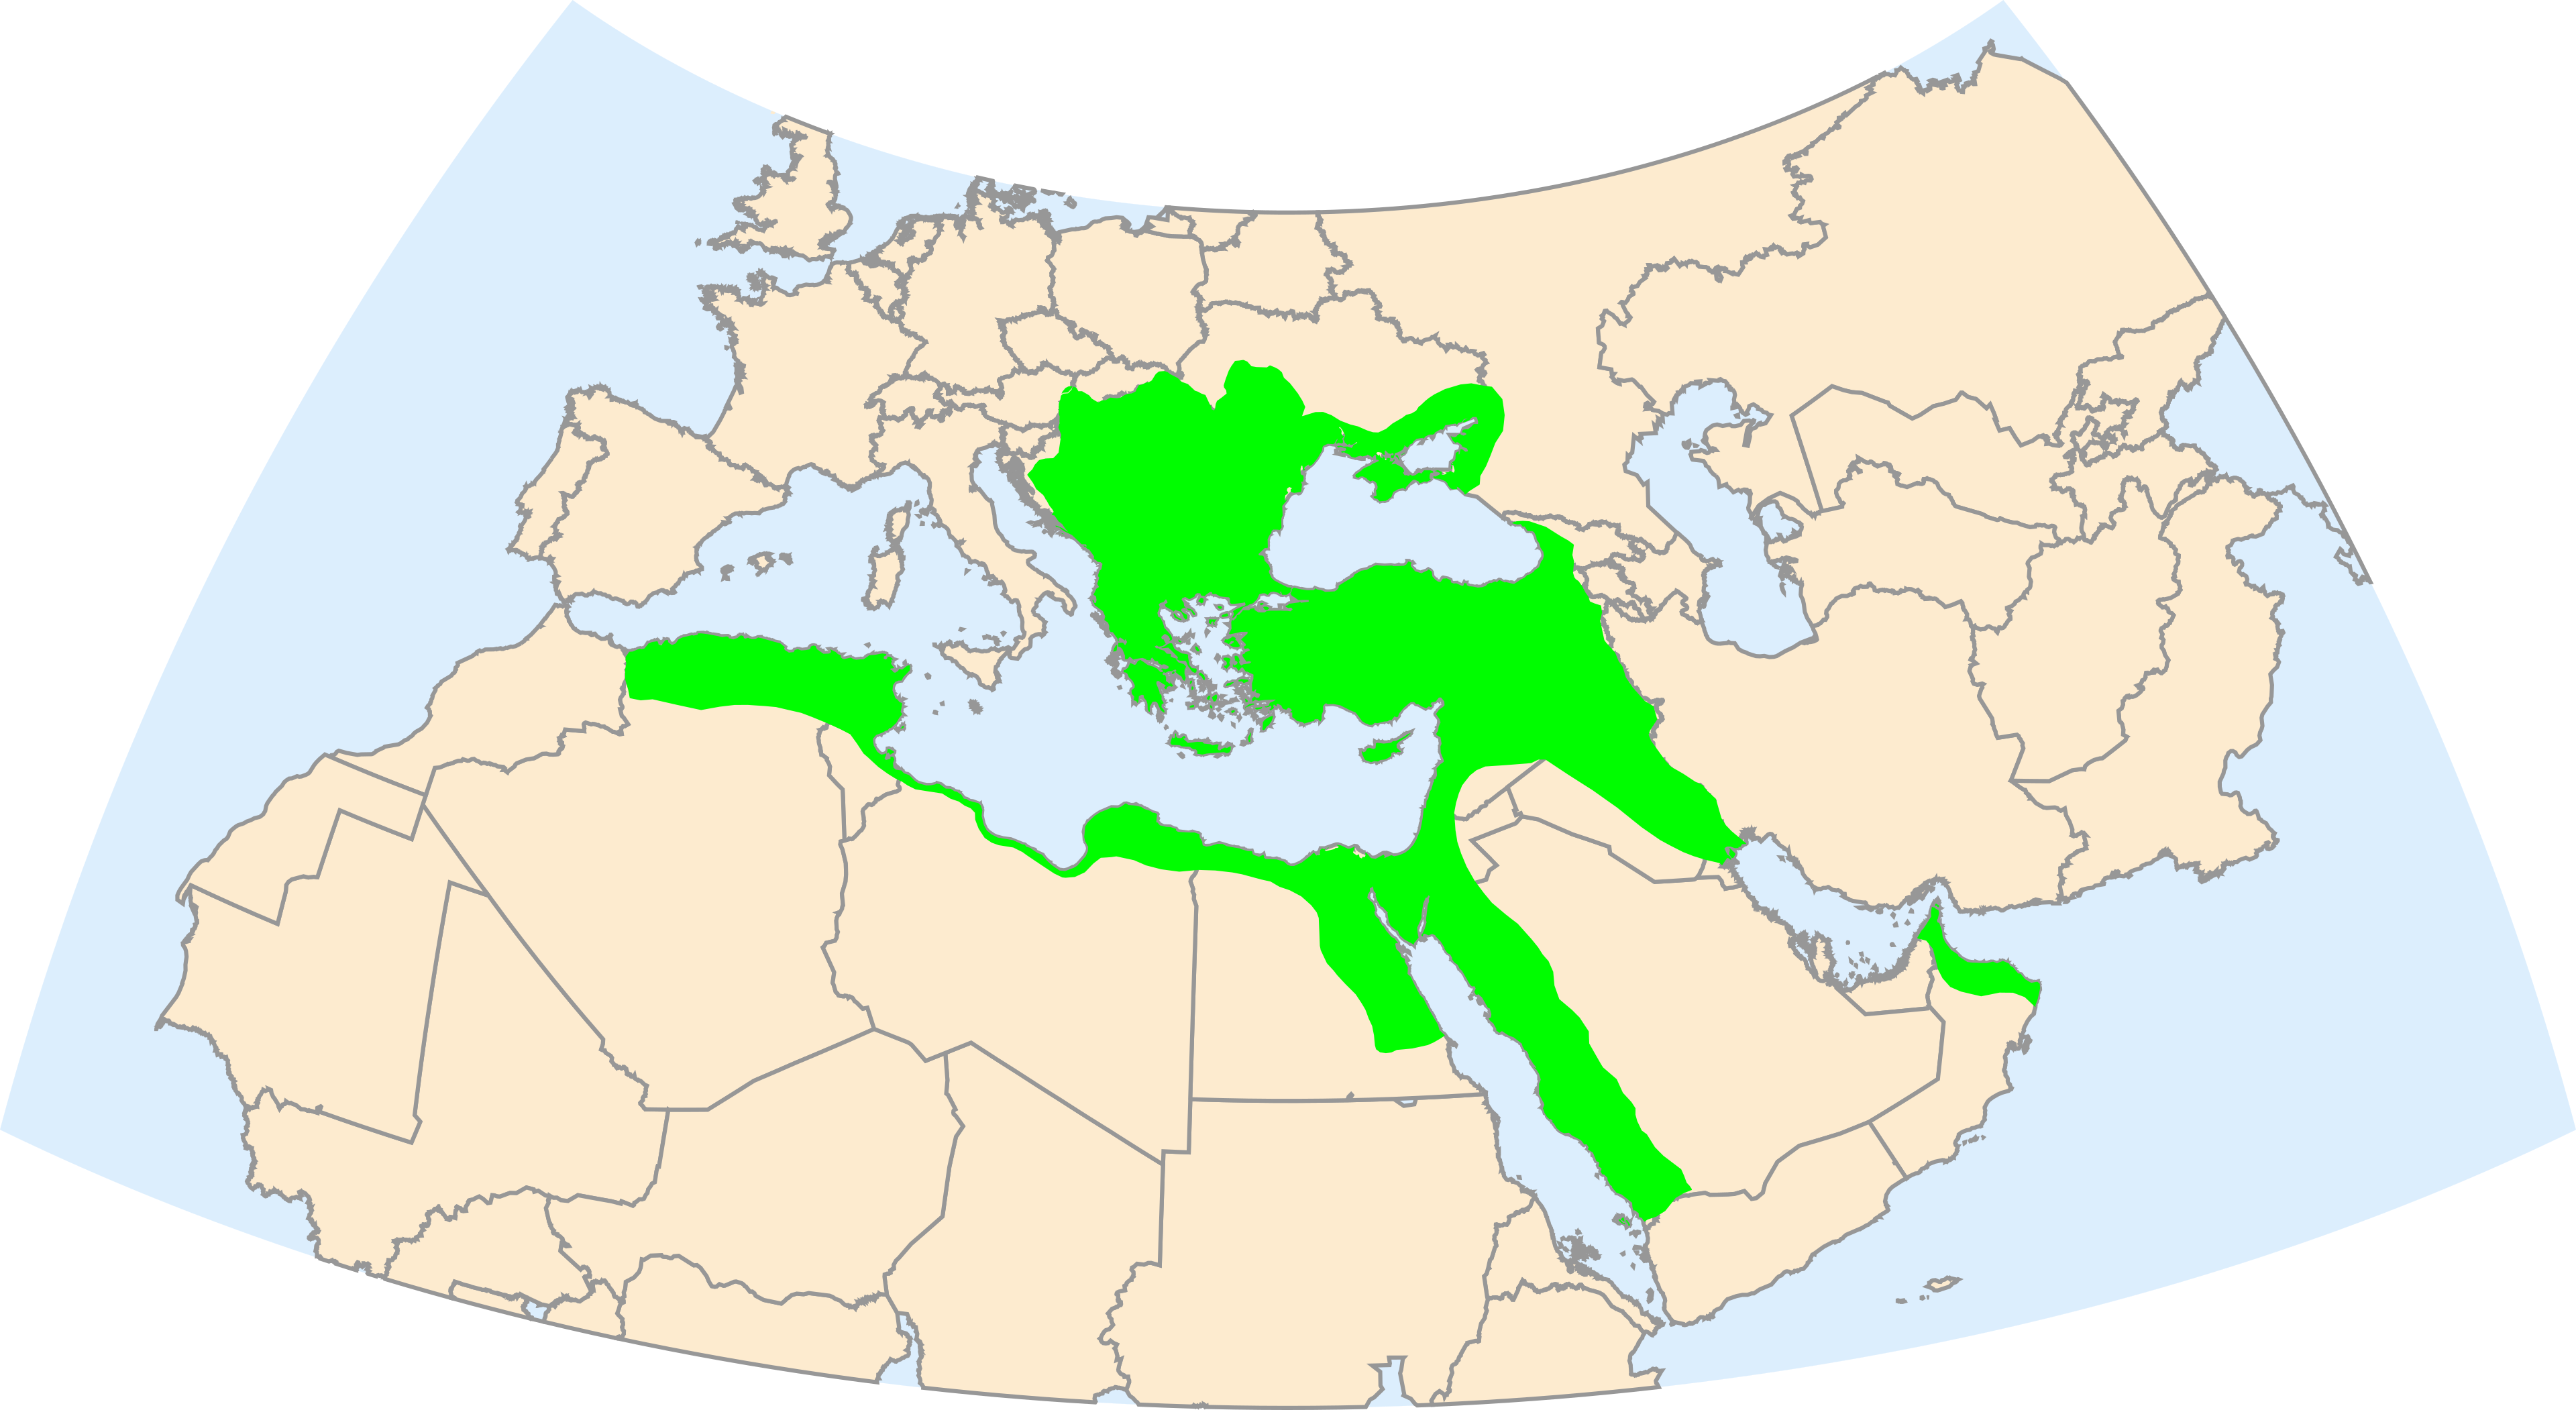
\includegraphics[width=1.4\textwidth]{1683OttomanEmpire.png}
			\end{figure}
			
	\end{columns}
\end{frame}

\section{Early 20\inst{th} Century}
\begin{frame}{Early 20\inst{th} Century}
	\begin{enumerate}
		\item Orient Express
		\item World War I
	\end{enumerate}
\end{frame}

\end{document}